% Activate the following line by filling in the right side. If for example the name of the root file is Main.tex, write
% "...root = Main.tex" if the chapter file is in the same directory, and "...root = ../Main.tex" if the chapter is in a subdirectory.
 
%!TEX root =  ../Thesis.tex

\chapter[Fit Strategy and Results]{Fit Strategy and Results}


Once the data has been sent through the trigger and cuts, it is still expected
that a large number of QCD events will remain, in which there might be a (probably comparatively small)
number of signal events.  The role of the fit is to mathematically describe
the distribution of the $m_{bb}$ of all the remaining events, and to enable the
possible extraction of a signal from the background.  

This general strategy is possible because the signal events are coming from a 
resonance, the $H/A$ particle, while the background consists of a smoothly 
falling spectrum owing to the fact that it comes from various QCD processes.
That means that $H/A$, if they are present, will show up as a bump in the $m_{bb}$
spectrum.  Using the signal MC, we define what we expect for the shape of
the signal resonance (the normalization is given to us by nature, and 
is a free parameter that must be extracted if the presence of signal is identified),
while the background fit is completely data-driven. The $m_{bb}^{'}$ distribution 
is fit in the background-dominated $bbanti$ region, and then those shapes 
are used as starting templates when fitting the background in the $bbb$ signal 
search region.  That templating process is tested in background MC to verify
that it does not introduce any bias from the $m_{bb}^{'}$ shapes differing
in the $bbb$ and $bbanti$ regions.
    
    
%The $m_{bb}$ ranges above
%and below the signal resonance, the mass sidebands, are used to 
%fit the background distribution to a polynomial, which can then be interpolated
%into the signal region.  That allows us to test the goodness-of-fit for a 
%background-only hypothesis against the fit quality for a signal+background
%hypothesis, for various signal normalizations.  

These fit results are then
the ingredients for the limit-setting procedure, which is detailed in the next section.

This chapter details the various categories that are used in the fit, and
the parametric forms that are used to fit them.   

\subsection{Fit Model and Categories}
\label{subsec:fitmodel}
The fit is performed in several different categories, which vary in the 
signal/background ratio, the signal and background shapes, and the
absolute normalizations of the signal and background.  In a situation like
this, where there are several categories that can be defined and the
search sensitivity varies depending on which category is being examined,
it can benefit the overall search sensitivity to fit each category 
separately and then combine them at the end.  While the parameteric form
of the fit (for both signal and background) is the same in each category (histograms fit over the range
-50$<m_{bb}^{'}<$350 GeV, in bins of 40 GeV), the signal is fit separately
in each $n_{jets}$ and $b$-tag category.  The background is fit
separately in bins of $n_{jets}$, but the shape is constrained to be the
same in all $b$-tag categories for a given number of jets.  This constraint
helps with convergence and has minimal chance of signal contamination
biasing the fit, since in practice the background fit is heavily dominated
by the high-statistics $bbanti$ control region.

The statistical analysis of the data employs an unbinned likelihood
function, defined as:
\begin{equation}
\text{Pois}(N|\mu S+B) \prod_{k=1}^{njet\ cat} \prod_{l=1}^{N_{tag\ cat}} \prod_{i=1}^{N_{l}} \left[ \mu N_{S,k,l} PDF_{sig,k,l}(m_{bb,i}) + N_{B,k,l} PDF_{bkg}(m_{bb,i}) \right]
\end{equation}
where:
\begin{itemize}
\item the product is over the $b$-tag categories $l$, the n$_{jets}$ categores $k$, and over the events in each category $i$;
\item $N_{S,l}$ and $N_{B,l}$ are the expected signal and background yield in each category;
\item $PDF_{sig,l}(m_{bb})$ and $PDF_{bkg}(m_{bb})$ are the signal and background probability density functions for  the different categories;
\item $\mu$ is a signal strength which multiplies the overall signal prediction.
\end{itemize}


The $b$-tag fit categories $l$ are the three exclusive categories to which events are assigned
based on the $b$-tag value of the third-most $b$-jet-like jet in the event (the two most
$b$-like jets have already been $b$-tagged in the trigger, and are assumed to be true
$b$-jets).  These are the categories outline in Section~\ref{sec:background_strategy}: 
\textit{bbb}, \textit{bbloose}, and \textit{bbanti}. 




The second type of categorization is based on the number of 
jets in the event: 3, 4, or 5 or more jets.  We find that the signal
shape can change based on the number of events, as well as the overall
signal and background normalizations.  For more details on the effect of 
the number of jets on the signal distributions, see Section~\ref{sec:n_jets_sig}. 



\subsection{Signal Yield Tests in Signal+Background Scenario}
An important cross-check is that the signal+background model returns the correct background
and, especially, signal yields that are present in the dataset that is being fit.
We need to check both the zero-signal case, verifying that the signal yield found
by the fit is consistent with zero, and a number of nonzero signal cross sections,
checking that the cross-section found by the fit comes back bias-free. 

The zero-signal results are tabulated in Table~\ref{tab:spurious_signal}; the 
signal yields returned by the fit are extremely close to zero (when restricting
ourselves to 3 or fewer significant figures, they round to 0.0 for all mass points)
with a statistical error that decreases with $m_A$.

%that it could introduce bias in the form of spurious signal ($N_{sp}$), or signal that is 
%not really ``there'' but is found by the signal+background fit anyway when fitting over the 
%full mass range.  To test for this possibility, we run the signal+background fit over
%samples of events that do not have any signal present, to see if the fit
%returns a signal yield that is consistent with zero.  Those results are tabulated
%in Table~\ref{tab:spurious_signal}.

 
\begin{table}
    \center
    \caption{The signal cross sections (in pb) returned by the signal+background fit
    to a background-only distribution
    \label{tab:spurious_signal}}
    \begin{tabular}{ c c } \hline \hline
        $m_A$ & signal returned (pb) \\ \hline
        400 GeV & 0.0$\pm$0.86 \\
        450 GeV & 0.0$\pm$0.87 \\
        500 GeV & 0.0$\pm$0.63 \\
        550 GeV & 0.0$\pm$0.50 \\
        600 GeV & 0.0$\pm$0.38 \\
        650 GeV & 0.0$\pm$0.29 \\
        700 GeV & 0.0$\pm$0.17 \\
        800 GeV & 0.0$\pm$0.12 \\
        \hline
    \end{tabular}
\end{table} 


We similarly try injecting signals of various cross sections, to see if 
the fit still returns the correct cross section when signal is present.
\textbf{those tests are ongoing, but looking very encouraging.  Testing
cross sections of 1-10 pb, we see biases of approx. 20\% but believe
those come from an approximation in how some errors are computed.
We are currently building an series of tests based on toy MC generation
to verify that the fit is not, in fact, biased when the errors are
treated correctly, which they would be in data and also toy MC. Once
those tests are complete, we'll tabulate them here. }


Some example results of these fits, with injected signals of 0, 3, and 10 pb, can 
be seen for 450 GeV and 700 GeV mass points in Figures~\ref{fig:signal_injection_450}
and ~\ref{fig:signal_injection_700}.


\begin{figure}[hbt]
    \center
    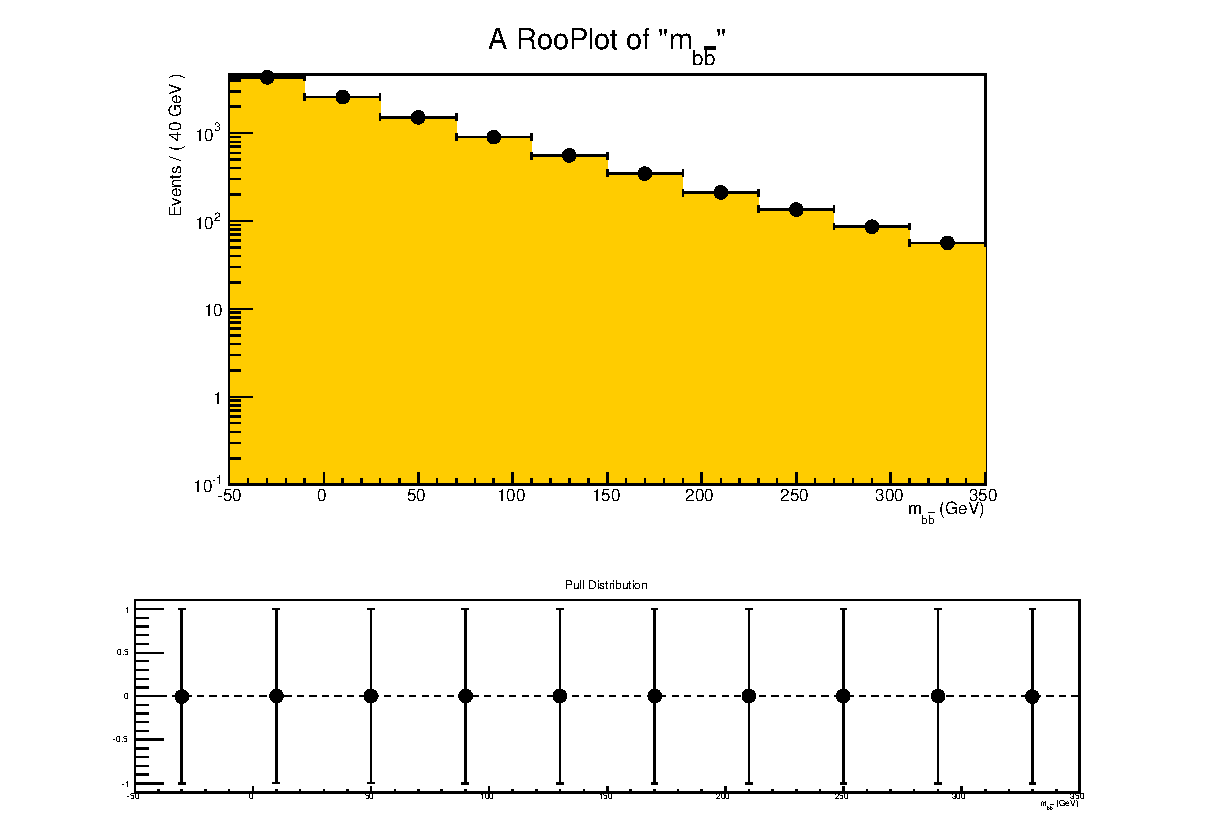
\includegraphics[width=0.3\linewidth]{FitResults/images/fitData_bAbb_450_log_3jets_bbb_hipt_0sig.eps}
    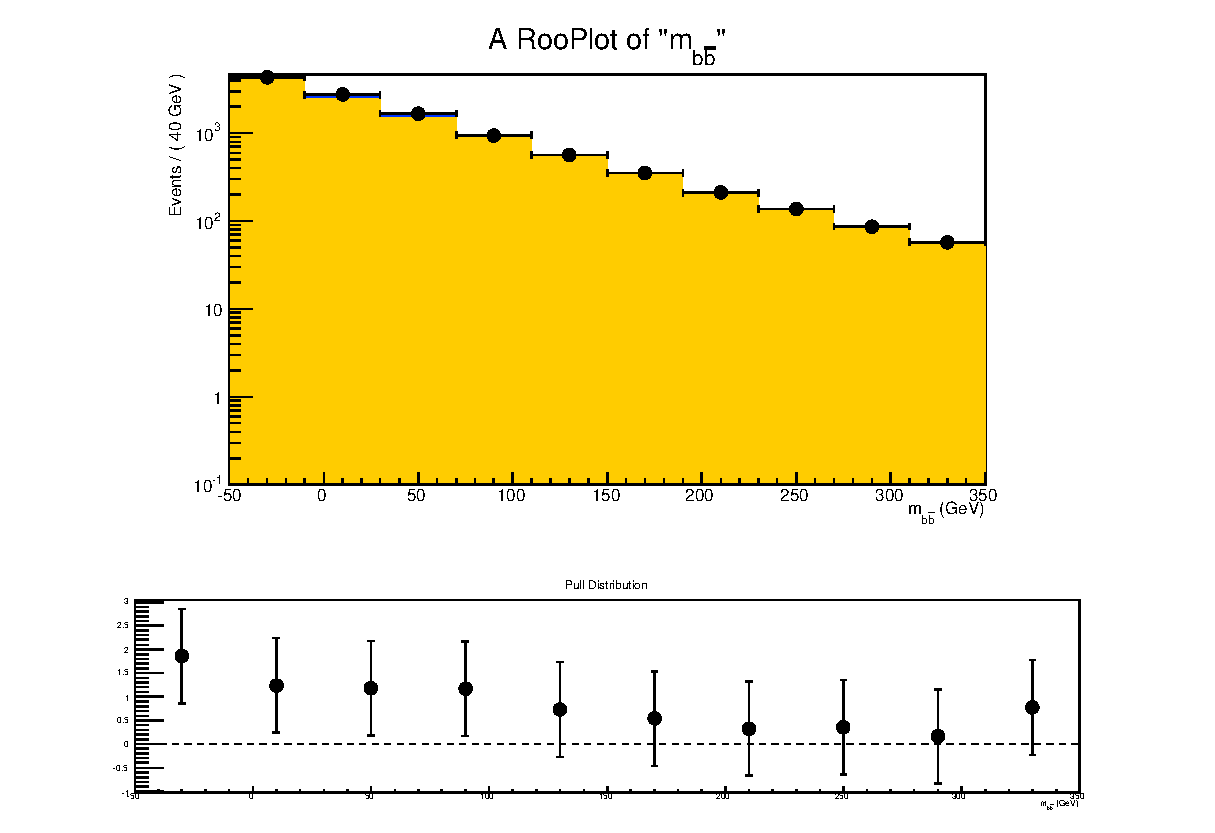
\includegraphics[width=0.3\linewidth]{FitResults/images/fitData_bAbb_450_log_3jets_bbb_hipt_3sig.eps}
    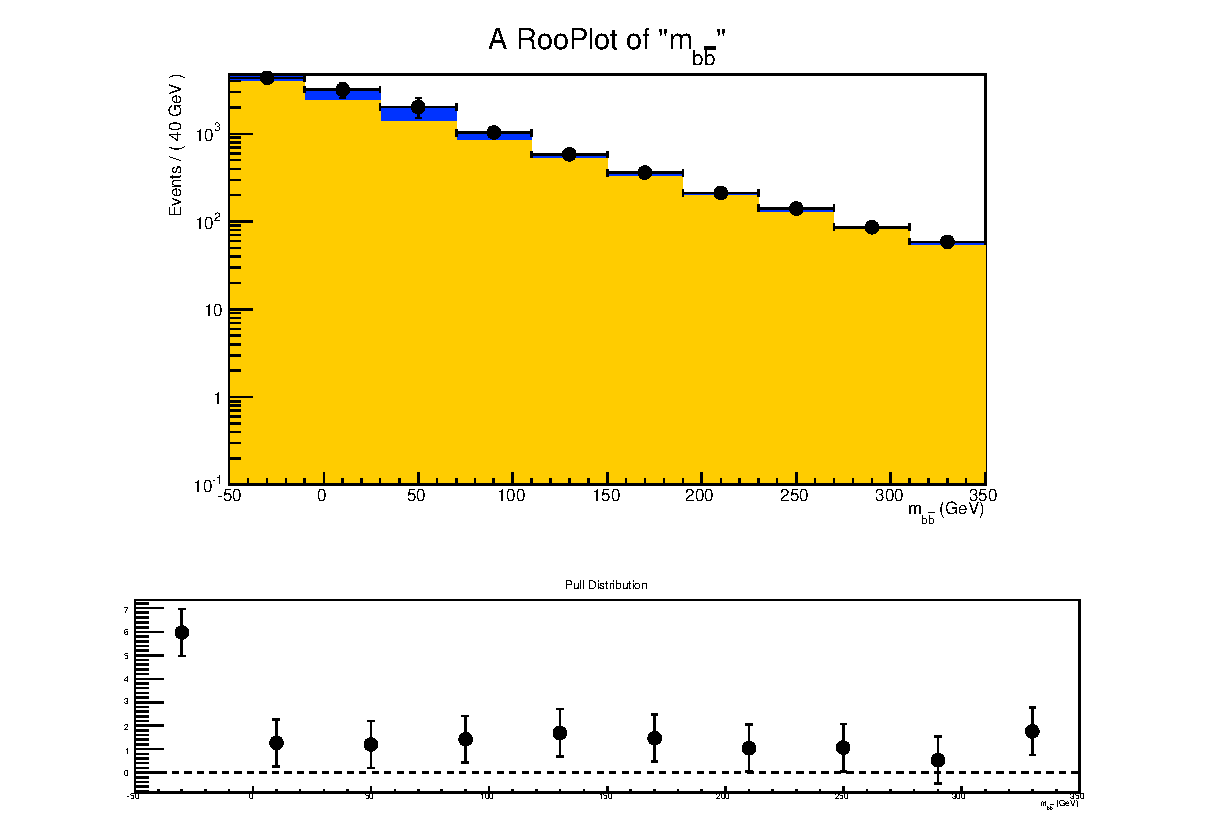
\includegraphics[width=0.3\linewidth]{FitResults/images/fitData_bAbb_450_log_3jets_bbb_hipt_10sig.eps}
    \caption{Examples of a signal+background fit when looking for a 450 GeV Higgs boson,
    when signal events are injected with a cross section $\times$ branching ratio of 0, 3, and 10 pb.
    The ``data'', including background and injected signal, is the data points with the error bars,
    while the background component of the fit is visible in orange and the signal component of fit
    is the blue histogram.  The bin-by-bin pull plots compare the background-only fit to the ``data''
    distribution. \textbf{known bug with the error bars on the signal fit, so errors on the pulls aren't
    to be trusted right now}
    \label{fig:signal_injection_450}}
\end{figure}

\begin{figure}[hbt]
    \center
    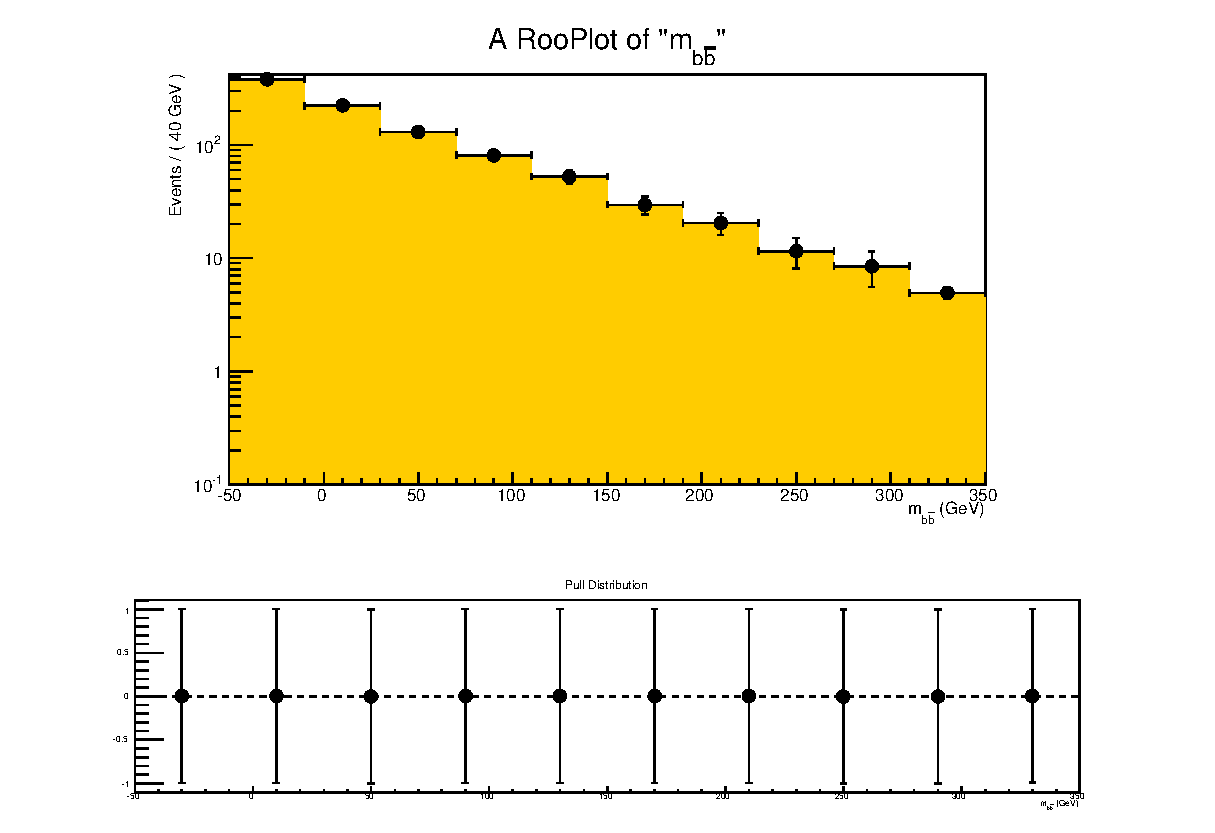
\includegraphics[width=0.3\linewidth]{FitResults/images/fitData_bAbb_700_log_3jets_bbb_hipt_0sig.eps}
    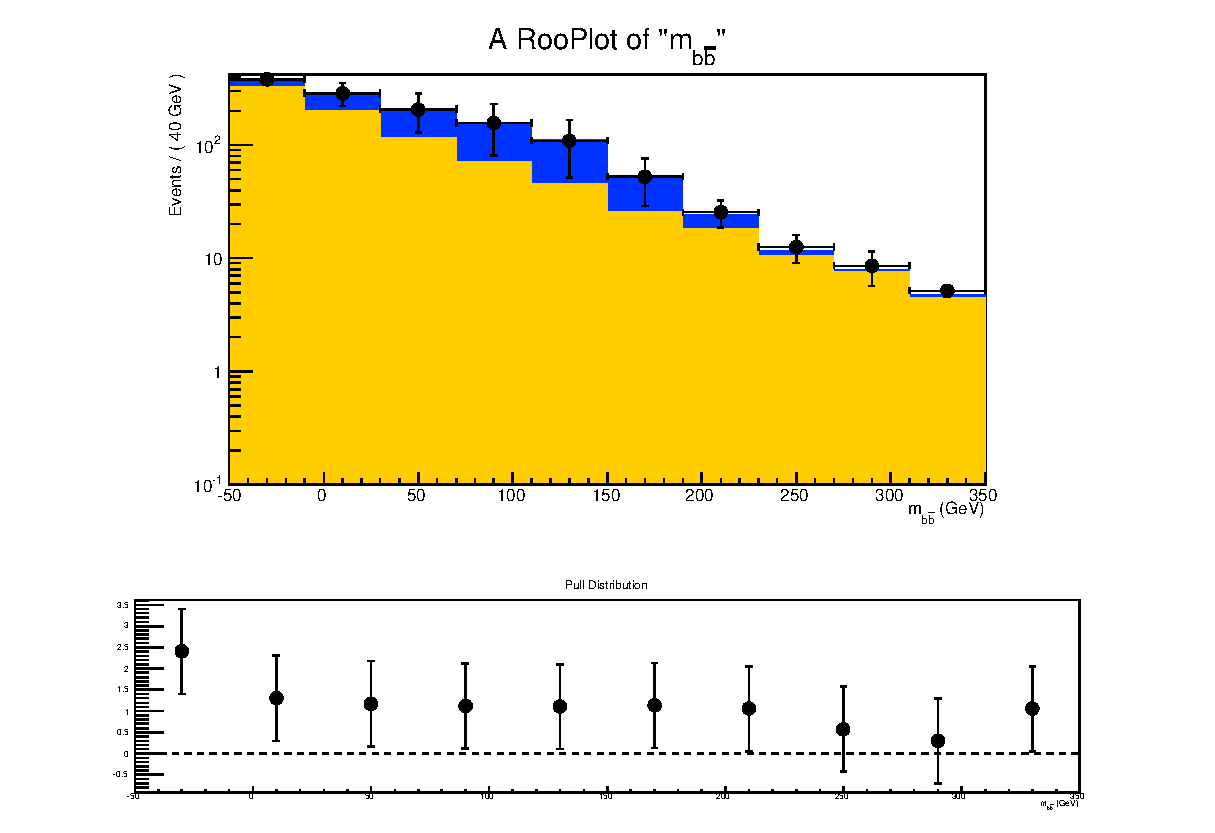
\includegraphics[width=0.3\linewidth]{FitResults/images/fitData_bAbb_700_log_3jets_bbb_hipt_3sig.eps}
    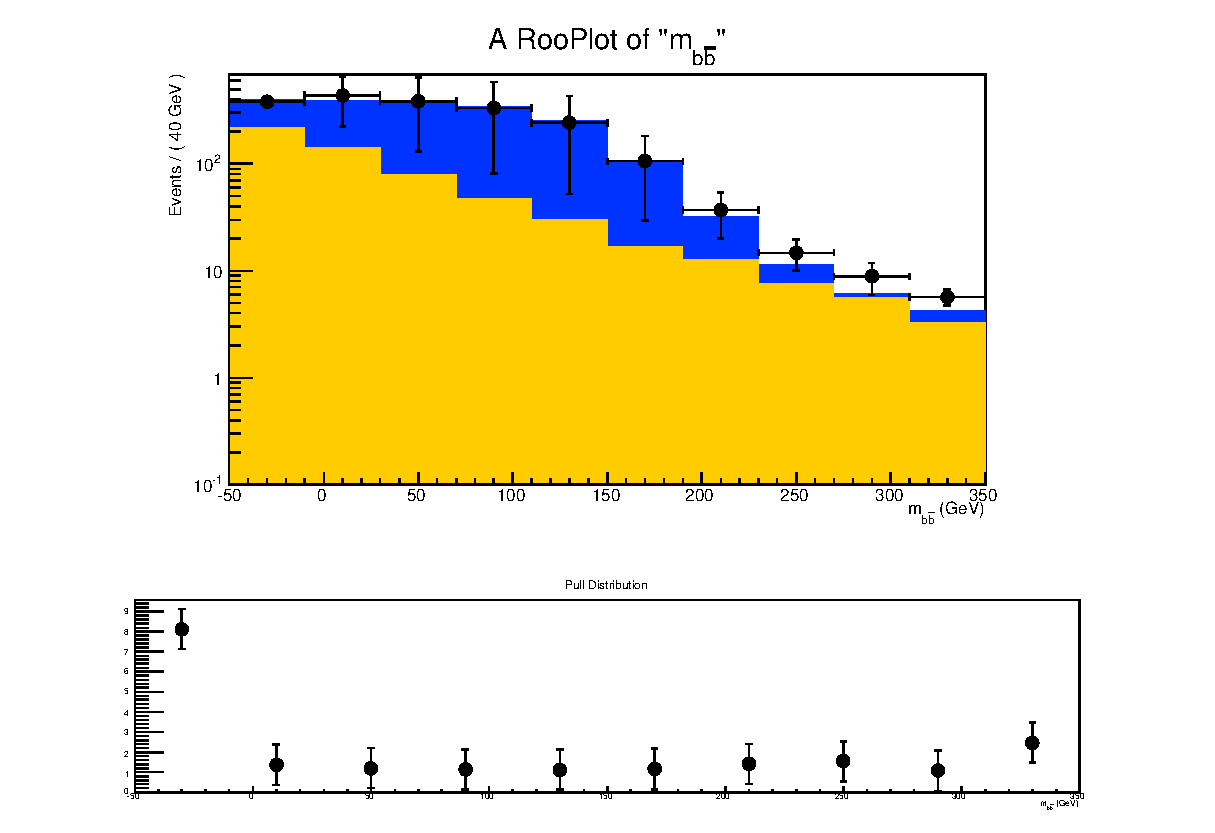
\includegraphics[width=0.3\linewidth]{FitResults/images/fitData_bAbb_700_log_3jets_bbb_hipt_10sig.eps}
    \caption{Examples of a signal+background fit when looking for a 700 GeV Higgs boson,
    when signal events are injected with a cross section $\times$ branching ratio of 0, 3, and 10 pb.
    The ``data'', including background and injected signal, is the data points with the error bars,
    while the background component of the fit is visible in orange and the signal component of fit
    is the blue histogram.  The bin-by-bin pull plots compare the background-only fit to the ``data''
    distribution. \textbf{known bug with the error bars on the signal fit, so errors on the pulls aren't
    to be trusted right now}
    \label{fig:signal_injection_700}}
\end{figure}


%\begin{table}
%    \center
%    \caption{The best-fit parameter values for the 2-parameter exponential background
%    function, of the form $f(x)=e^{-x/\tau+\omega x^2}$, for the each of the 9 
%    fit categories (3 tag categories times 3 jet categories).  
%    \label{tab:bkgFit}}
%    \begin{tabular}{ c p{3cm} p{3cm} } \hline \hline
%        category & 1-parameter exponential $\chi^2/DOF$ & 2-parameter exponential $\chi^2/DOF$ \\ \hline
%        \textit{bbb} 3 jet & 1.5 & 1.1 \\
%        \textit{bbb} 4 jet & 0.9  & 0.7 \\
%        \textit{bbb} 5+ jet & 0.9  & 0.7 \\
%        \textit{bbloose} 3 jet & 0.8 & 0.6 \\
%        \textit{bbloose} 4 jet & 1.2 & 0.7 \\
%        \textit{bbloose} 5+ jet & 1.5 & 1.1 \\
%        \textit{bbanti} 3 jet & 3.9 & 1.0 \\
%        \textit{bbanti} 4 jet & 3.9 & 1.2 \\
%        \textit{bbanti} 5+ jet & 2.8 & 1.2 \\
%        \hline
%    \end{tabular}
%\end{table} 






\section{Limit Extraction}
Once the signal and background have been fit, the CL$_s$ method is used to 
determine the $\sigma\times BR$ that can be excluded at the 95\% confidence
level \cite{CLS1}, \cite{CLS2}, \cite{CLS3}.  The CL$_s$ method is a
frequentist limit-setting procedure that is designed to give upper limits that
are greater than the true value of $\sigma\times BR$ with a probability of at
least 95\%.

Once the signal and background PDF shapes are determined in the fit,
the limit setting procedure proceeds as follows.  The fits are used to generate
an ensemble of toy MC datasets
that are combined into a single representative dataset, called the ``Asimov
dataset'' for that distribution.  Then 
in order to obtain the nominal fit result in terms of $\mu$ and $\sigma_{\mu}$
the likelihood function is maximized with respect to all parameters.
This is referred to as the maximized log-likelihood value MLL.
The test statistic $q_\mu$ is then constructed according to
the profile likelihood:
\begin{equation}
q_\mu = 2 \mathrm{ln} (\mathcal{L} (\mu,
\hat{\hat{\theta_\mu}})/\mathcal{L} (\hat{\mu}, \hat{\theta})), 
\end{equation}
where
$\hat{\mu}$ and $\hat{\theta}$ are the parameters that maximize the
likelihood (with the constraint $0 \leq \hat{\mu} \leq \mu$), and
$\hat{\hat{\theta}}_\mu$ are the nuisance parameter values that maximize the
likelihood for a given $\mu$. This test statistic is used to measure
the compatibility of the background only model with the observed
data. 

Expected exlusion limits following this procedure are shown in Fig.~\ref{fig:limitSensitivity} and Table
~\ref{tab:limitSensitivity}. %These are obtained under the assumption that
% a good estimate of the background parameters is given by the fit values reported in Table~\ref{tab:bkgFit}. 
\textbf{these are preliminary plots, which will change a bit as the 
systematics get more fully integrated into the fits}

\begin{table}
    \center
    \caption{The expected production cross sections times branching ratios
        to be excluded at 95\% CL, along with the 1-sigma and 2-sigma statistical uncertainties 
    \label{tab:limitSensitivity}}
    \begin{tabular}{ c c c c c c } \hline \hline
        mass point & expected limit (pb) & -2$\sigma$ & -1$\sigma$ & +1$\sigma$ & +2$\sigma$ \\ \hline 
        400 GeV & 1.68 & 0.92 & 1.21 & 2.33 & 3.13 \\
        450 GeV & 1.79 & 0.96 & 1.29 & 2.48 & 3.33 \\
        500 GeV & 1.30 & 0.69 & 0.93 & 1.81 & 2.42 \\
        550 GeV & 0.97 & 0.53 & 0.70 & 1.36 & 1.82 \\
        600 GeV & 0.75 & 0.40 & 0.54 & 1.03 & 1.39 \\
        650 GeV & 0.57 & 0.30 & 0.41 & 0.79 & 1.05 \\
        700 GeV & 0.49 & 0.27 & 0.36 & 0.69 & 0.92 \\
        800 GeV & 0.37 & 0.20 & 0.27 & 0.51 & 0.69 \\


%        \textit{bbb} 3 jet & 1.5 & 1.1 \\
%        \textit{bbb} 4 jet & 0.9  & 0.7 \\
%        \textit{bbb} 5+ jet & 0.9  & 0.7 \\
 %       \textit{bbloose} 3 jet & 0.8 & 0.6 \\
%        \textit{bbloose} 4 jet & 1.2 & 0.7 \\
%        \textit{bbloose} 5+ jet & 1.5 & 1.1 \\
%        \textit{bbanti} 3 jet & 3.9 & 1.0 \\
%        \textit{bbanti} 4 jet & 3.9 & 1.2 \\
%        \textit{bbanti} 5+ jet & 2.8 & 1.2 \\
       \hline
    \end{tabular}
\end{table} 




\begin{figure}[hbt]
\center
\includegraphics[width=0.9\linewidth]{FitResults/SMHiggs_ZH_v62.eps}
\caption{The expected 95\% excluded $\sigma\times$BR as a function of $m_A$, 
for 400$<m_A<$800 GeV.
\label{fig:limitSensitivity}}
\end{figure}

